\clearpage
\section*{Supplementary material}
\footnotesize
\subsection*{S1. Concepts, stems and the word forms they match (1 Nov 1884--1888, both papers)}
Stems are matched as substrings of surface forms; following \citet{schoots2023b} we inspected forms for false positives (our first \emph{law} stem also matched \emph{inteto}, speech, and was dropped) but did not hand-filter them, so run-together forms (e.g. \emph{rulumenteningomsebenzi}) and missed variants remain. All stems, forms and glosses await review by a first-language isiXhosa speaker; e.g.\ \emph{rulumente} is glossed `government' here but `parliament' by Schoots et al.\ (2023a, p.~62). Political concepts were fixed before testing; religion was suggested by the classifier and is exploratory.\\[2pt]
\begin{tabular}{@{}p{1.9cm}p{1.6cm}p{2.0cm}p{9.6cm}@{}}
\toprule
Concept & Type & Stems & Most frequent matched forms (count; number of distinct forms) \\ \midrule
parliament & political & palamente & palamente (1754), ipalamente (47), palamenteni (22), epalamente (14), bapalamente (1), nepalamente (1), yepalamente (1); 11 forms \\
vote & political & voti & ivoti (301), voti (217), evotini (136), abavoti (98), ngevoti (55), levoti (22), nevoti (22); 115 forms \\
government & political & rulumente, rulumeni & rulumente (1882), rulumeni (1336), rulumenteni (7), urulumente (5), urulumeni (3), rulumenini (2), serulumente (1); 14 forms \\
rule & political & mbuso & zombuso (169), umbuso (76), mbuso (60), yombuso (42), kombuso (37), lombuso (28), kulombuso (23); 43 forms \\
law & political & mteto & umteto (724), lomteto (475), mteto (406), ngomteto (167), ngumteto (94), komteto (76), nomteto (76); 82 forms \\
rights & political & lungelo & amalungelo (315), ilungelo (288), lungelo (113), nelungelo (54), namalungelo (50), lilungelo (39), elilungelo (37); 115 forms \\
country & political & lizwe & lizwe (646), ilizwe (292), kwelilizwe (201), elilizwe (101), elizwe (96), belilizwe (76), yelilizwe (52); 78 forms \\
land & political & mhlaba & umhlaba (836), mhlaba (208), lomhlaba (156), nomhlaba (105), komhlaba (99), somhlaba (95), yomhlaba (94); 135 forms \\
freedom & political & kululek & inkululeko (27), kukululekile (24), ukululekile (13), ngenkululeko (10), abakululekileyo (8), nkululeko (8), nenkululeko (7); 92 forms \\
humanity & political & buntu & ubuntu (45), yobuntu (14), nobuntu (8), sobuntu (8), buntu (7), lobuntu (7), zobuntu (6); 29 forms \\
time & neutral & xesha & ixesha (787), ngexesha (364), xesha (298), amaxesha (243), lixesha (191), ngamaxesha (149), zamaxesha (114); 207 forms \\
house & neutral & ndlu & indlu (719), izindlu (328), kwindlu (276), ndlu (234), yendlu (227), ngendlu (133), nendlu (130); 193 forms \\
rain & neutral & mvula & imvula (267), mvula (31), yemvula (23), ezimvula (17), lemvula (16), yimvula (14), zimvula (10); 45 forms \\
cattle & neutral & nkomo & inkomo (555), zenkomo (258), nkomo (193), yenkomo (93), nenkomo (75), ngenkomo (35), lenkomo (33); 79 forms \\
religion & exploratory & tixo, kristu, krestu & tixo (684), kristu (207), krestu (118), makristu (7), kristukazi (7), makrestu (6), mkrestu (5); 32 forms \\
\bottomrule
\end{tabular}

\subsection*{S2. Secondary framing tests across settings}
Percentile of the observed shift among 2000 frequency-matched word sets, and one-sided $p$ (uncorrected). Jaccard = shift in a word's ten nearest neighbours (neighbour overlap; \citealp{gonen2020}). P+V = \emph{palamente} + \emph{voti}; P+V+R adds \emph{rulumente} (uncertain meaning). Directional $\Delta$: Isigidimi minus Imvo, religious minus political similarity (in $z$-score units), political concepts, two-sided $p$ against matched sets; the last columns give the control \emph{house}. Three settings survive Bonferroni over five ($p<0.01$): window 1, window 2, and window 2 with forms joined. Joining partly disjunctive forms (\emph{uku ba}) leaves the global profile gap unchanged. Matched sets are re-drawn for each test; without \emph{land} the pooled set is smaller, so lower power may contribute to the higher $p$.\\[2pt]
\begin{tabular}{@{}lcccccccccc@{}}
\toprule
Setting & P+V profile & P+V Jaccard & P+V+R profile & P+V+R Jaccard & $\Delta$ & $\Delta$ $p$ & $p$ w/o land & house $\Delta$ & house $p$ \\ \midrule
window 1 (tuned) & 92 ($p$=0.083) & 96 ($p$=0.039) & 92 ($p$=0.077) & 99 ($p$=0.007) & +0.68 & $<$0.001 & 0.010 & +1.08 & $<$0.001 \\
window 1, forms joined & 99 ($p$=0.010) & 95 ($p$=0.053) & 100 ($p$=0.001) & 100 ($p$=0.002) & +0.44 & 0.016 & 0.088 & +1.15 & $<$0.001 \\
window 2 & 86 ($p$=0.139) & 94 ($p$=0.061) & 90 ($p$=0.096) & 99 ($p$=0.010) & +0.76 & $<$0.001 & 0.045 & +1.34 & $<$0.001 \\
window 2, forms joined & 91 ($p$=0.094) & 98 ($p$=0.023) & 99 ($p$=0.011) & 100 ($p$=0.002) & +0.58 & 0.009 & 0.064 & +1.51 & $<$0.001 \\
window 5 & 62 ($p$=0.382) & 98 ($p$=0.016) & 81 ($p$=0.189) & 100 ($p$=0.002) & +0.66 & 0.015 & 0.256 & +0.84 & 0.061 \\
\bottomrule
\end{tabular}

\subsection*{S3. Era drift: does a concept's rate move across eras within one paper?}
Per-million-token rates and ratios (later/earlier, or Imvo/Isigidimi) with issue-bootstrap 95\% CIs.\\[2pt]
\begin{tabular}{@{}llrrl@{}}
\toprule
Concept & Comparison & First & Second & Ratio (95\% CI) \\ \midrule
parliament & Isigidimi: later / earlier era & 214 & 394 & 1.84 (0.96--4.98) \\
parliament & Imvo: later / earlier era & 1320 & 758 & 0.57 (0.50--0.66) \\
parliament & Imvo 1889-94 / Isigidimi 1876-83 (held-out) & 214 & 758 & 3.54 (1.98--9.58) \\
government & Isigidimi: later / earlier era & 2197 & 1095 & 0.50 (0.39--0.64) \\
government & Imvo: later / earlier era & 2234 & 1649 & 0.74 (0.67--0.81) \\
government & Imvo 1889-94 / Isigidimi 1876-83 (held-out) & 2197 & 1649 & 0.75 (0.65--0.88) \\
vote & Isigidimi: later / earlier era & 72 & 614 & 8.55 (3.51--18.94) \\
vote & Imvo: later / earlier era & 799 & 921 & 1.15 (0.88--1.51) \\
vote & Imvo 1889-94 / Isigidimi 1876-83 (held-out) & 72 & 921 & 12.82 (7.85--25.92) \\
religion & Isigidimi: later / earlier era & 2541 & 1678 & 0.66 (0.50--0.86) \\
religion & Imvo: later / earlier era & 445 & 612 & 1.38 (1.08--1.76) \\
religion & Imvo 1889-94 / Isigidimi 1876-83 (held-out) & 2541 & 612 & 0.24 (0.20--0.30) \\
\bottomrule
\end{tabular}

\subsection*{S4. Anchors for the directional test}
Anchors are the 15 top-PMI neighbours of each seed pair in held-out text (Isigidimi 1876-83 + Imvo 1889-94), frozen before testing. Religious (15 words; seeds \emph{tixo}, \emph{kristu}): \emph{sikelela}, \emph{sindisa}, \emph{ukumkanikazi}, \emph{inkosazana}, \emph{buka}, \emph{oyingcwele}, \emph{lilizwi}, \emph{msindisi}, \emph{nelizwi}, \emph{kwelizwi}, \emph{wanga}, \emph{lika}, \emph{yesu}, \emph{izono}, \emph{yehova}. Political (15 words; seeds \emph{palamente}, \emph{voti}): \emph{emqulwini}, \emph{wonyulo}, \emph{lonyulo}, \emph{elugqatsweni}, \emph{eziqingata}, \emph{lokunyula}, \emph{kwesase}, \emph{lokuvota}, \emph{endlu}, \emph{kwamagama}, \emph{ukumela}, \emph{izayo}, \emph{ngalomteto}, \emph{nawupina}, \emph{kwabase}. Seed words cannot themselves be tested (Fig.~S1). Political anchors include \emph{endlu} (`in the house'), which might have favoured the neutral control \emph{house}; re-running without \emph{endlu} leaves both the political lean and \emph{house}'s lean in place (outputs/framing\_matched\_tests\_noendlu.csv), and \emph{ngalomteto}, which contains the \emph{law} stem. Glosses are unverified: two religious anchors (\emph{ukumkanikazi}, \emph{inkosazana}) may reflect royal rather than religious register, and several anchors on both sides (\emph{lika}, \emph{buka}; \emph{nawupina}, \emph{kwabase}, \emph{izayo}) may be grammatical rather than topical, consistent with narrow-window PMI capturing grammar. All await speaker review.
\normalsize

\subsection*{S5. Readers' letters versus the rest of each paper}
Letters are detected by src/12\_letters.py: a letter opens by addressing the editor (vocative \emph{mhleli} or \emph{mcokeli}, not \emph{u/ku/ngu mhleli}, which refer to him) or by asking for insertion (\emph{ndifakele}, \emph{kaundifakele}), and ends at the signature (a run of very short lines). A hand check of 30 random detections found 28 genuine letters; the errors were usifake umkala (horse advert: `put a bit on it'); no mhleli wepepa lama bhulu ('and the editor of the Boer paper'). Recall was not measured. Imvo is restricted to the months in which Isigidimi has text; CIs from 4000 issue resamples; rates are not tested against matched sets. Hits = concept uses.\\[2pt]
\begin{tabular}{@{}llrrrrrr@{}}
\toprule
Part & Concept & Isig.\ tokens & Isig.\ hits & Imvo tokens & Imvo hits & Imvo/Isig. & 95\% CI \\ \midrule
letters & parliament & 18,344 & 2 & 70,475 & 48 & 6.25 & 2.09--16.92 \\
letters & religion & 18,344 & 57 & 70,475 & 77 & 0.35 & 0.19--0.69 \\
letters & vote & 18,344 & 4 & 70,475 & 58 & 3.77 & 1.04--18.93 \\
letters & government & 18,344 & 13 & 70,475 & 161 & 3.22 & 1.67--9.62 \\
rest of paper & parliament & 268,319 & 111 & 936,998 & 1280 & 3.30 & 2.53--4.51 \\
rest of paper & religion & 268,319 & 424 & 936,998 & 370 & 0.25 & 0.17--0.37 \\
rest of paper & vote & 268,319 & 172 & 936,998 & 821 & 1.37 & 0.79--2.83 \\
rest of paper & government & 268,319 & 301 & 936,998 & 1906 & 1.81 & 1.47--2.28 \\
\bottomrule
\end{tabular}

\subsection*{S6. Which sense of \emph{umhlaba}?}
For every use of the land stem (\emph{mhlaba}) we look at the 10 tokens either side. Religious cues: \emph{izulu}, \emph{lizulu}, \emph{nezulu}, and words containing \emph{zulwini}, \emph{tixo}, \emph{kristu}, \emph{yesu}, \emph{msindisi}, \emph{ngcwele} (bare \emph{zulu} is excluded: \emph{kwa zulu} is Zululand). Property/political cues: words containing \emph{taitile}, \emph{mteto}, \emph{rulumente}, \emph{palamente}, \emph{mantyi}, \emph{fama}, \emph{voti}, \emph{nyulo}, \emph{rafu}, \emph{lokishi}. Most uses have neither cue. Example lines for a speaker to check are in outputs/land\_kwic.md.\\[2pt]
\begin{tabular}{@{}llrrr@{}}
\toprule
Paper & Cue & Uses & Share & 95\% CI \\ \midrule
Imvo & religious & 1408 & 0.9\% & 0.4--1.4\% \\
Imvo & property/political & 1408 & 26.8\% & 23.8--29.7\% \\
Isigidimi & religious & 353 & 3.4\% & 1.7--5.3\% \\
Isigidimi & property/political & 353 & 12.7\% & 8.5--17.7\% \\
\bottomrule
\end{tabular}

\subsection*{S7. Same editor, different control; same control, different editor}
Cells (editors after Schoots, 2023b, p.~71): Jabavu edits Isigidimi (Jan 1881--Oct 1884); Jabavu edits Imvo (Nov 1884--1888); Gqoba edits Isigidimi (Nov 1884--1888); Makiwane edits Isigidimi (1876--80; Stewart until 1876). Ratios of rates per million tokens; 95\% CIs from 4000 issue resamples; $p$: two-sided, against 2000 matched sets of random words (src/15\_editor\_control.py). Every contrast is also a contrast in time; \emph{rule} has only 9 uses in Jabavu's Isigidimi, so its large ratios are not interpreted.\\[2pt]
\begin{tabular}{@{}lrrrrrrrrr@{}}
\toprule
Concept & \multicolumn{3}{c}{Jabavu: Imvo / Isigidimi} & \multicolumn{3}{c}{Isigidimi: Gqoba / Jabavu} & \multicolumn{3}{c}{Isigidimi: 1881--84 / 1876--80} \\
 & ratio & 95\% CI & $p$ & ratio & 95\% CI & $p$ & ratio & 95\% CI & $p$ \\ \midrule
parliament & 1.69 & 1.23--2.54 & 0.088 & 0.50 & 0.33--0.79 & 0.043 & 49.86 & 14.41--405.79 & $<$0.001 \\
vote & 3.07 & 1.98--5.23 & 0.017 & 2.36 & 1.07--4.61 & 0.034 & 11.63 & 4.32--98.99 & 0.004 \\
government & 1.21 & 0.99--1.49 & 0.387 & 0.59 & 0.44--0.77 & 0.043 & 0.78 & 0.61--1.01 & 0.289 \\
rule & 19.47 & 9.46--77.40 & 0.001 & 8.28 & 3.57--31.56 & 0.009 & 0.38 & 0.09--1.32 & 0.228 \\
law & 1.36 & 1.08--1.72 & 0.235 & 0.80 & 0.53--1.17 & 0.376 & 1.31 & 0.98--1.76 & 0.314 \\
rights & 0.93 & 0.76--1.16 & 0.808 & 0.82 & 0.58--1.13 & 0.480 & 2.91 & 2.05--4.12 & 0.006 \\
country & 1.08 & 0.92--1.29 & 0.773 & 1.13 & 0.90--1.41 & 0.596 & 0.74 & 0.59--0.92 & 0.243 \\
land & 1.10 & 0.91--1.34 & 0.689 & 0.95 & 0.70--1.28 & 0.853 & 0.94 & 0.76--1.16 & 0.815 \\
freedom & 0.68 & 0.51--0.92 & 0.443 & 0.95 & 0.64--1.38 & 0.899 & 1.52 & 1.01--2.42 & 0.408 \\
humanity & 0.97 & 0.59--1.90 & 0.959 & 1.88 & 0.98--3.88 & 0.227 & 0.97 & 0.45--1.96 & 0.967 \\
religion & 0.37 & 0.27--0.50 & 0.025 & 1.38 & 1.03--1.83 & 0.168 & 0.35 & 0.26--0.47 & $<$0.001 \\
\bottomrule
\end{tabular}

\subsection*{S8. Hyper-parameter search for the embeddings}
fastText skip-gram, tuned on text outside the test window (Isigidimi 1876--83, Imvo 1889--94) so that tuning never sees the compared years. Criterion: seed stability, the mean top-10 nearest-neighbour overlap between two runs that differ only in random seed \citep{antoniak2018}; unstable embeddings would turn noise into apparent shifts. 34 settings over dimension (50, 100, 200, 300, 400), window (1, 2, 3, 5, 8) and epochs (10, 20, 30), searched in rounds that extended the grid past each optimum. Chosen: dimension 400, window 1, 20 epochs. Stability is highest at the narrowest window, which favours grammar over topic; the paper therefore also reports windows 2 and 5 (Table S2). Best setting per window:\\[2pt]
\begin{tabular}{@{}rrrrrr@{}}
\toprule
Window & Dimension & Epochs & Isigidimi 1876--83 & Imvo 1889--94 & Mean stability \\ \midrule
1 & 400 & 20 & 0.844 & 0.814 & 0.829 \\
2 & 300 & 20 & 0.823 & 0.798 & 0.810 \\
3 & 300 & 20 & 0.810 & 0.799 & 0.805 \\
5 & 400 & 20 & 0.798 & 0.796 & 0.797 \\
8 & 200 & 10 & 0.758 & 0.755 & 0.757 \\
\bottomrule
\end{tabular}\\[2pt]
At the chosen setting, word2vec reaches a stability of 0.64 against fastText's 0.83, so fastText is used throughout.

\subsection*{S9. Tokenizer cost}
Each condition is a random sample of about 100{,}000 words. Modern text is the isiXhosa section of MasakhaNEWS \citep{adelani2023}. The old-spelling condition is the same modern sample with the aspiration marks of modern orthography removed by fixed rules (\emph{th}$\to$\emph{t}, \emph{kh}$\to$\emph{k}, \emph{ph}$\to$\emph{p}, \emph{rh}$\to$\emph{r}, \emph{ch}$\to$\emph{c}, \emph{qh}$\to$\emph{q}, \emph{xh}$\to$\emph{x}; src/05\_fertility.py), so only spelling changes and the words stay the same: it is compared per word. Historical text differs in word division, so it is compared per 100 characters. The politics/business sample checks genre within modern news: its cost is close to all modern news, while both 1880s papers cost more, so the historical penalty is not simply a news-topic effect, though 1880s and modern newspapers still differ in genre. 95\% CIs from bootstrap resampling are within $\pm$0.01 subwords per word.\\[2pt]
\begin{tabular}{@{}lrrrrrrr@{}}
\toprule
Condition & Words & \multicolumn{2}{c}{XLM-R} & \multicolumn{2}{c}{Serengeti} & \multicolumn{2}{c}{mBERT} \\
 & & per word & per 100 ch. & per word & per 100 ch. & per word & per 100 ch. \\ \midrule
Modern news & 100,003 & 2.613 & 35.28 & 1.867 & 25.21 & 3.040 & 41.05 \\
Modern news, old spelling & 100,003 & 2.555 & 35.56 & 1.909 & 26.57 & 2.937 & 40.88 \\
Modern news, politics/business only & 88,389 & 2.673 & 35.21 & 1.888 & 24.88 & 3.116 & 41.06 \\
Isigidimi 1884--88 & 100,013 & 2.259 & 36.71 & 1.743 & 28.33 & 2.569 & 41.75 \\
Imvo 1884--88 (matched draw) & 100,006 & 2.240 & 36.92 & 1.738 & 28.65 & 2.533 & 41.75 \\
\bottomrule
\end{tabular}

\renewcommand{\thefigure}{S\arabic{figure}}\setcounter{figure}{0}
\begin{figure}[h]\centering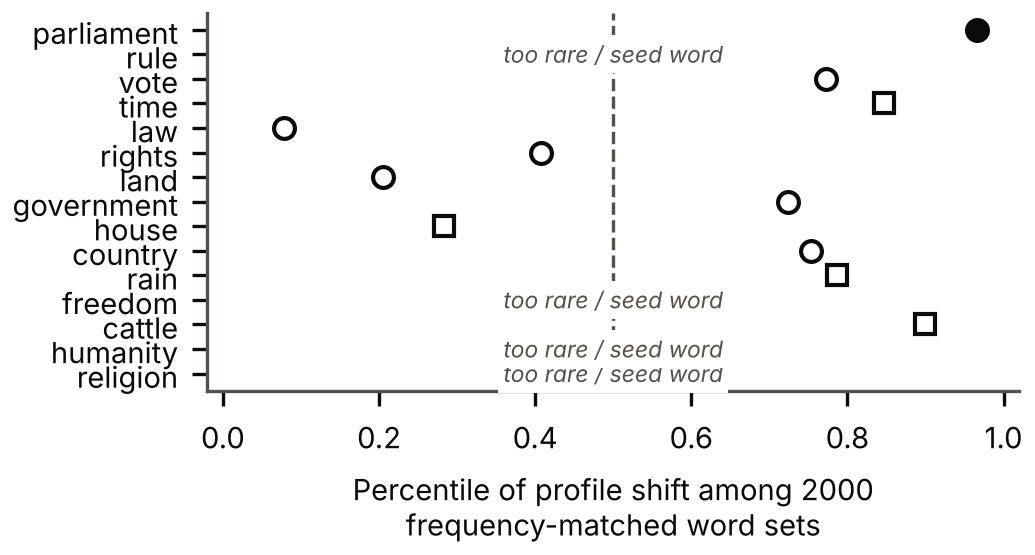
\includegraphics[width=3.45in]{fig_framing.png}
\caption{Profile-shift percentile of each concept among matched sets (markers as in Fig.~1, left); `too rare' = too few occurrences, `seed word' = anchor source, untestable.}\end{figure}
\begin{figure}[h]\centering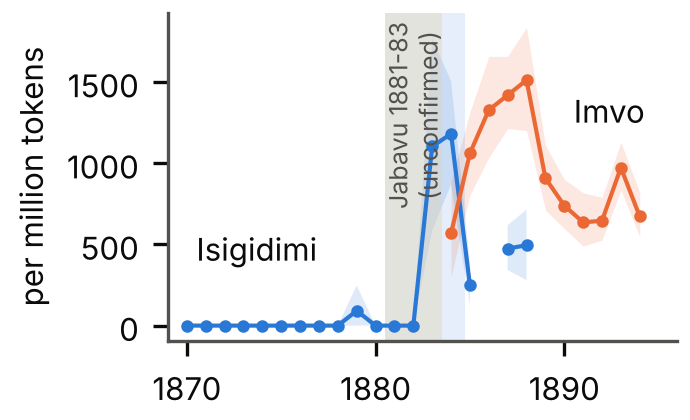
\includegraphics[width=2.3in]{fig_parliament_by_year.png}
\caption{Parliamentary vocabulary per million tokens; it enters Isigidimi in 1883 (light blue: twice-monthly issues, Schoots et al., 2023a, p.~59).}\end{figure}
